\documentclass[conference]{IEEEtran}
\IEEEoverridecommandlockouts
% The preceding line is only needed to identify funding in the first footnote. If that is unneeded, please comment it out.
\usepackage{cite}
\usepackage{amsmath,amssymb,amsfonts}
\usepackage{algorithmic}
\usepackage{graphicx}
\usepackage{textcomp}
\usepackage{xcolor}
\usepackage{graphicx} % for \includegraphics command
\usepackage{float} % for [H] option to force figure placement
\def\BibTeX{{\rm B\kern-.05em{\sc i\kern-.025em b}\kern-.08em
    T\kern-.1667em\lower.7ex\hbox{E}\kern-.125emX}}
\begin{document}

\title{Paper Title*\\
{\footnotesize \textsuperscript{*}Note: Sub-titles are not captured in Xplore and
should not be used}
\thanks{Identify applicable funding agency here. If none, delete this.}
}

\author{\IEEEauthorblockN{1\textsuperscript{st} Given Name Surname}
\IEEEauthorblockA{\textit{dept. name of organization (of Aff.)} \\
\textit{name of organization (of Aff.)}\\
City, Country \\
email address}
\and
\IEEEauthorblockN{2\textsuperscript{nd} Given Name Surname}
\IEEEauthorblockA{\textit{dept. name of organization (of Aff.)} \\
\textit{name of organization (of Aff.)}\\
City, Country \\
email address}
\and
\IEEEauthorblockN{3\textsuperscript{rd} Given Name Surname}
\IEEEauthorblockA{\textit{dept. name of organization (of Aff.)} \\
\textit{name of organization (of Aff.)}\\
City, Country \\
email address}
}

\maketitle

\begin{abstract}
This document is a model and instructions for \LaTeX.
This and the IEEEtran.cls file define the components of your paper [title, text, heads, etc.]. *CRITICAL: Do Not Use Symbols, Special Characters, Footnotes, 
or Math in Paper Title or Abstract.
\end{abstract}

\begin{IEEEkeywords}
component, formatting, style, styling, insert
\end{IEEEkeywords}

\section{Introduction}
In recent years, the scientific focus has shifted towards the next generation of mobile computing—wearable devices. This shift has spurred significant advancements in egocentric vision. Among its various applications, first-person or “egocentric” perception using wearable cameras has the potential to alleviate cognitive overload and provide users with a superhuman personal episodic memory. By capturing and indexing what we see in meaningful and easily accessible ways, these devices could transform how we interact with our environment.

This purpose is embodied by the Natural Language Query (NLQ) task in the Ego4D Episodic Memory benchmark. The NLQ challenge involves taking a natural language query and a video clip, and identifying the exact temporal segment in the camera wearer's past footage that contains the answer \cite{b1}. These types of problems are referred to as Natural Language Video Localization (NLVL) problems.

The task can be approached in two ways: as a video segment matching problem, where the goal is to find the best matching segment given a query \cite{b2}, or as a regression problem, which directly predicts the boundaries of the relevant video segment \cite{b3}.

The NLQ challenge, along with related video-language question answering tools, has gained considerable attention from the research community. However, the task presents several technical challenges. Firstly, videos may be of arbitrary length, which raises the question of how to build models that can reason over a long temporal range. Secondly, integrating video and text modalities remains a complex issue.

In this paper, we propose an approach that first solves the NLVL problem by extracting the start and end boundaries of the answer span from the video. Then, we exploit a Video Question Answering (VideoQA) model to generate a natural language answer from the extracted clip.

As a baseline, we first address the NLVL task with a standard span-based QA framework for video input named VSLBase, comparing the outcomes obtained using different sets of pre-extracted features. We then propose an improved version, VSLNet, implemented with different encoders to assess the most effective version. Finally, we utilize an open-source model, Video-LLaVA, to generate answers in natural language.

\section{Related work}

\subsection{Localizing Video Segments with Natural Language}

The task of localizing moments within a long video has grown enormously in the last few years. Prior work was solely based on scanning videos by predefined windows of different sizes. Gao et al. (2017) introduced the first dataset, "TACoS," for temporal activity localization with sentence descriptions, utilizing a sliding window approach. These methods typically generate segment candidates throughout the video using temporal sliding windows. These segments are then either compared (Hendricks et al. 2017) or combined (Gao et al. 2017) with the given sentence to identify the relevant parts of the video. While these models achieve good overall matching between video segments and sentences, they often miss fine-grained interactions and context details, and are inefficient due to the exhaustive search process across the video's timeline, making them computationally expensive \cite{b4}.

With the advancement of deep learning, models that jointly learn video and language representations have become more prominent. In \cite{b5} Anne Hendricks et al. (2018) developed a model using temporal attention mechanisms to improve localization accuracy. This model explicitly reasons about different temporal segments in a video, highlighting the importance of temporal context for localizing phrases that include temporal language. However, these models are sensitive to negative samples and need to densely sample candidate moments to achieve good performance, resulting in low efficiency and limited flexibility.

Recent methods often use transformers to jointly model the interactions between video and language modalities. These models leverage self-attention mechanisms to capture complex relationships between frames in a video and words in a sentence. Mun et al. (2020) developed a multi-modal transformer model that captures interactions between video frames and language features more effectively, resulting in better performance for NLVL tasks. Ghosh et al. (2019) proposed a cross-modal transformer network that processes both video and text data using separate transformer encoders and then integrates the information to perform localization tasks.

In this paper, we closely follow the model proposed by Hao et al. in \cite{b3}, which treats the input video as a text passage, transforming NLVL into a standard span-based QA problem. VSLBase adopts a simple and standard span-based QA framework, facilitating the modeling of differences between video and text through the addition of extra modules. The VSLNet addresses these differences by introducing the QGH module.



\subsection{Large Language Visual Models}
Recent advancements in natural language processing have extended the capabilities of large language models (LLMs) to comprehend not only textual data but also visual content. One notable approach involves mapping images into text-like tokens, which allows LLMs to process both text and images in a unified manner. This integration of visual and textual information enables LLMs to understand and generate responses based on visual input.

Several of these new architectures leverage pre-trained large language models to build unified models for multi-modality. For instance, Flamingo [Alayrac et al., 2022] employs a frozen vision encoder and large language model, using gated cross-attention to fuse vision and language modalities, demonstrating impressive few-shot capabilities. BLIP-2 [Li et al., 2023] introduces Q-Former to align visual features from the frozen visual encoder with large language models such as Flan-T5 [Chung et al., 2022] and OPT [Zhang et al., 2022]. Additionally, PaLM-E [Driess et al., 2023] integrates features from sensor modalities directly with PaLM [Chowdhery et al., 2022].

In this paper, we examine Video-LLaVA, a robust baseline for LLVM that manages both images and videos simultaneously. Like MiniGPT-4 \cite{b6}, Video-LLaVA pre-aligns image and video features, but also conducts joint training of images and videos, enabling LLMs to develop multi-modal reasoning capabilities from a unified visual representation.

Despite their strengths, these models face limitations due to their reliance on frozen visual backbones, which may result in suboptimal alignment because of the restricted parameter set. To address these shortcomings, mPLUG-Owl \cite{b7} has been introduced. This model not only aligns representations between vision and language foundation models for enhanced knowledge acquisition and real-world grounding but also excels in understanding language and multi-modal instructions.


\section{Dataset}
Traditional computer vision systems have relied on third-perspective images for a very long time. Addressing this limitation, the Ego4D dataset represents a revolutionary leap in the field of first-person visual perception. Ego4D comprises of a total of 3670 hours of egocentric video footage captured by 931 different participants across 74 locations worldwide. This dataset, created by Facebook AI (now Meta AI) in collaboration with numerous academic institutions and research organizations, is the most diverse and curated collection of daily-life activities to date, including household chores, leisure activities, work tasks and more. 

To mitigate overfitting, Ego4D employs seven different head-mounted cameras, capturing a broader spectrum of human behavior and interactions than previous datasets. Additionally, it introduces five benchmark challenges aimed at testing and enhancing AI systems' capabilities in first-person perception. These challenges include episodic memory (recall past events and interactions), forecasting (predicting future actions and events) hand-object interaction(recognizing hand movements and object manipulations), (recognizing hand movements and object manipulations), audio-visual diarization(differentiating speakers and sounds) and social interaction (analyzing behaviours and interactions). 

Our focus is on the Episodic memory challenge, which aims to evaluate and advance AI systems’ capabilities to understand and recall past events from egocentric video data. Specifically, it addresses queries expressed in natural language, with responses providing temporal windows for observing or inferring answers. To approach this task, the dataset provides extensive annotations which include:

\begin{itemize}
    \item \textbf{Detailed timestamps}: since in ego4d videos are divided into shorter segments called clips, annotations specify start and end timestamps for segments within individual video clips and in relation to the entire video.
    \item \textbf{Language queries}: Each annotation includes formulated questions aimed at extracting specific information from the video content.
    \item \textbf{Temporal information}: Queries are accompanied by temporal data indicating their occurrence within both the clip and the overall video, along with the “response track” in the video.
    \item \textbf{Template descriptions}: Annotations provide a set of 13 template questions, with designated slots for variables such as objects and actions, meant to span things a user might ask to augment their memory. In figure 1 we report the distribution of queries per template.
    \item \textbf{Raw tags}: Included to capture the essence of the queries, aiding in processing and analysis of the annotated data.
\end{itemize}

\begin{figure}[h]
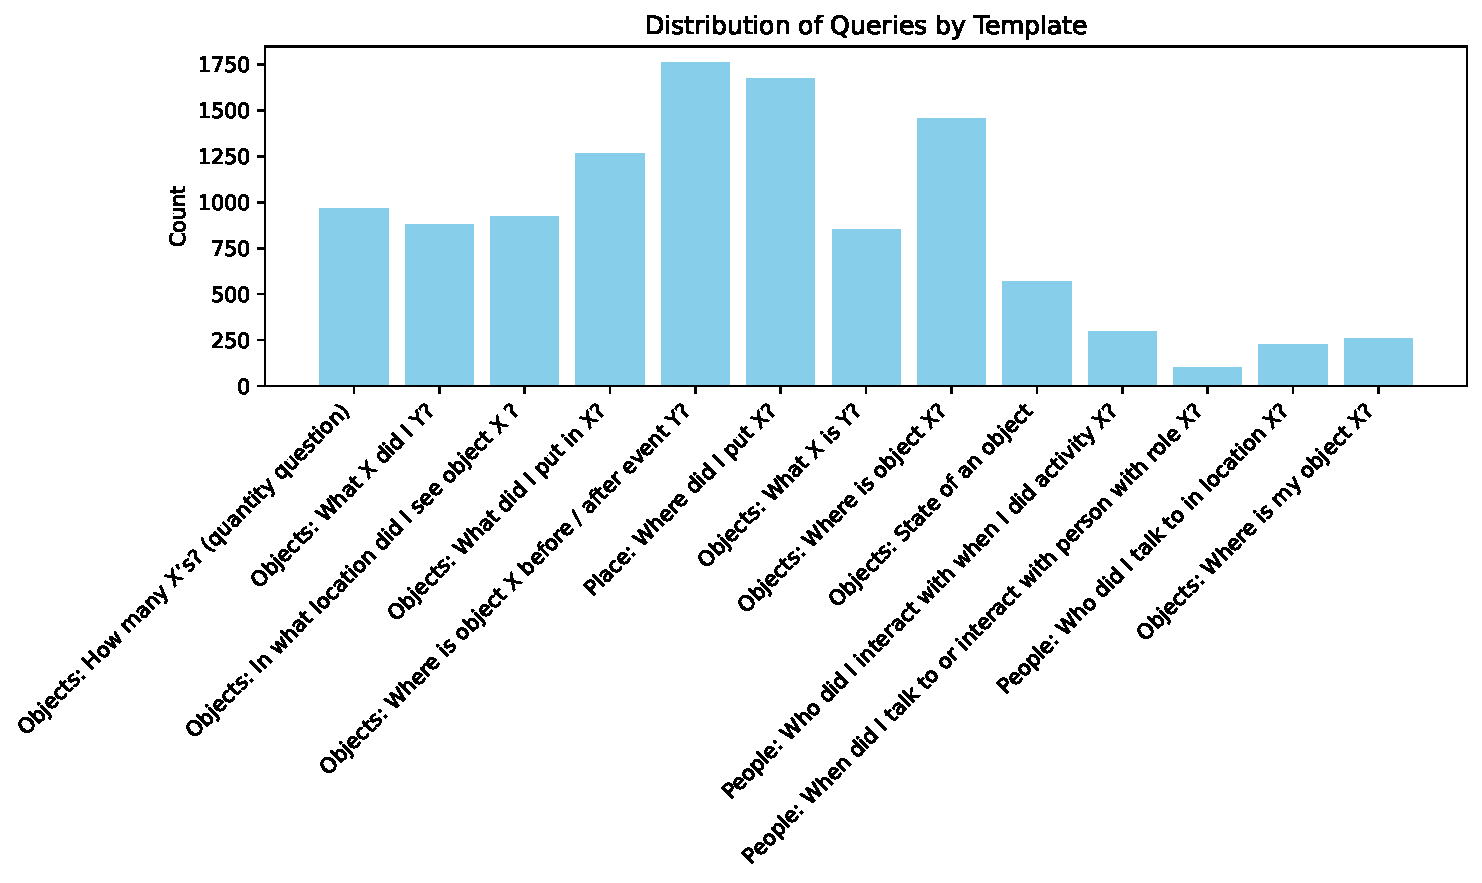
\includegraphics[width=0.4\textwidth]{Figure1.pdf} % adjust width as needed
\caption{Caption}
\label{fig:figure2}
\end{figure}

Analyzing the data retrieved through annotations yields valuable insights for our current task. Initially, we note that the average duration of clips is 522 seconds, with the majority lasting 480 seconds (or 8 minutes). Approximately 9.01\% of the dataset consists of short queries, defined as lasting four frames or less at a frame rate of 30 frames per second; these queries of approximately 0 seconds duration are excluded.

Another observation from plotting the distribution is the relative duration of each query compared to the total duration of its corresponding video clip. It's evident that most queries cover 2\% or less of the total clip duration. Additionally, the average response interval, when plotted, shows a value of 9.67 seconds.

In Figure 2 reported below, we illustrate the distribution of the number of queries per video, suggesting an average of 15 queries per video.

\begin{figure}[h]
\centering
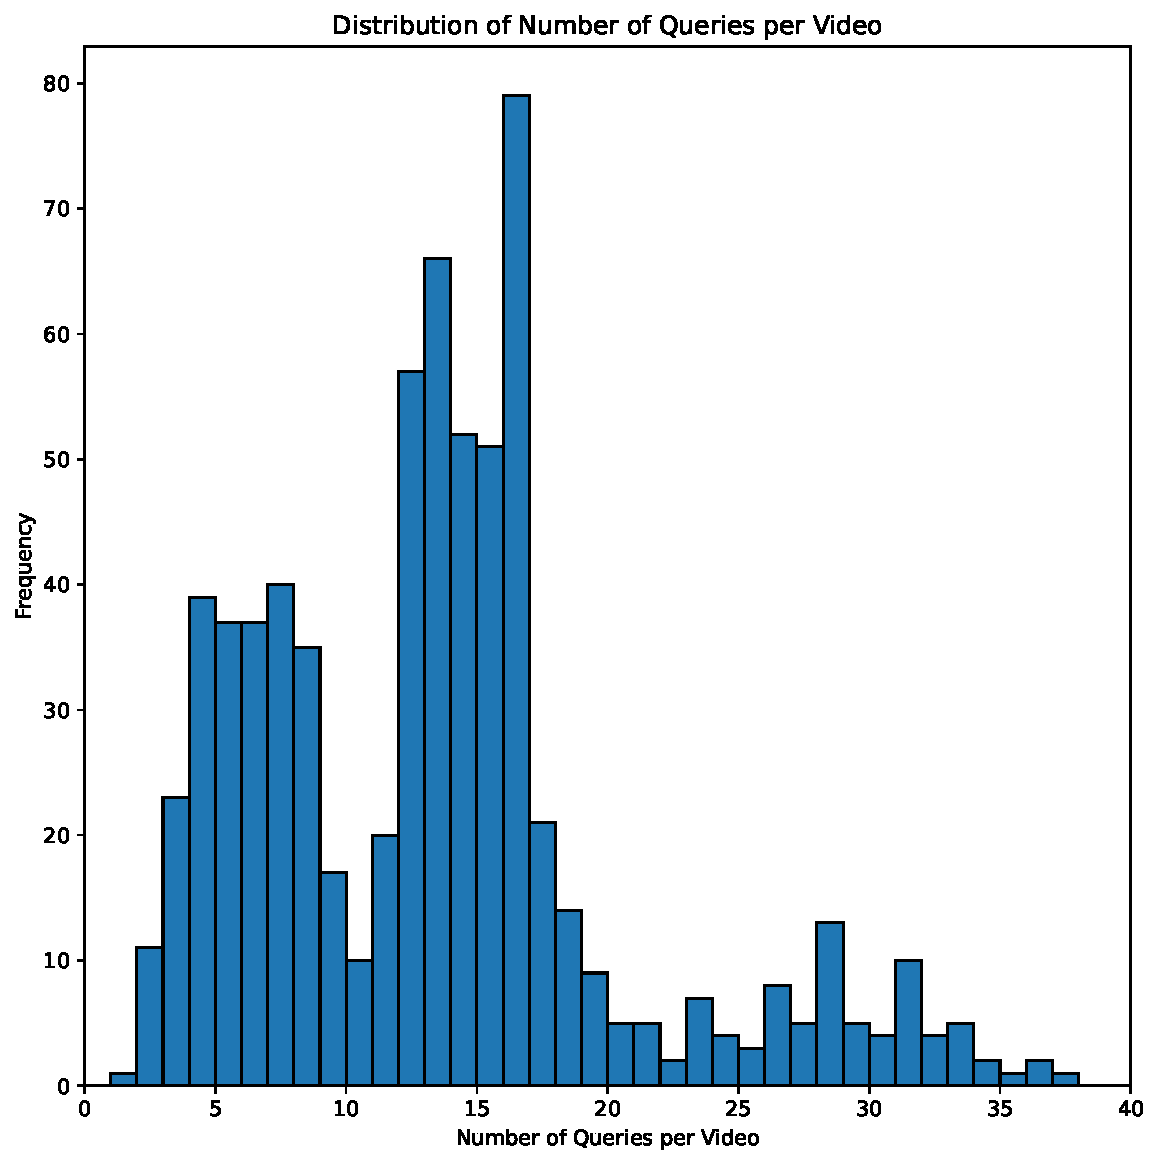
\includegraphics[width=0.4\textwidth]{Figure2.pdf} % adjust width as needed
\caption{Caption}
\label{fig:figure2}
\end{figure}

\section{Proposed Approach}
\subsection{Task}
With the NLQ task, we are able to retrieve only the information about the temporal interval of the video that answers the input query. To also return a textual answer, which could be more useful for the user, we need to use VLMs (Video Language Models).\\

For VLMs, it is computationally expensive to process the entire video to answer the query. Therefore, to counter this computational cost, the proposed approach leverages the strengths of both models. We use the NLQ as the first step of a pipeline to identify the short interval of interest. Then, we can cut the entire video to the interval of interest and feed it to a VLM alongside the query, instead of using the entire clip.\\

Another approach could be to aggregate the full video information to make it more feasible for the model. However, this could lead to a loss of detail.\\

The pipeline we used is shown in fig.\ref{fig:fullPipeline}, and for the VLM task, we chose Video-LLaVA.

\subsection{Video-LLava}
Video LLava is a Large Vision-Language model, so given a query and a visual input, its task is to produce a textual answer.  It is capable of simultaneously handling both image and videos. Many existing approaches encode images and videos into separate input spaces, but this can be a limitation. Instead, this model uses a unified visual representation for both modalities within the language feature space.\\
Also, in paper [citare paper 4] it is shown that unified visual representation befits LLMs in learning both images and videos when compared to models specifically designed for one of the modalities.
\subsubsection{Model Structure}
The first step consists in extracting visual features (from videos or images). For this purpose, LanguageBind encoders are used [citare paper]. These encoders can map different modalities into the textual feature space. At the end of this process, we obtain a unified visual representation.\\ 
The next step is to use a shared projection layer to project the features, after that they are in the same space with the tokenized textual queries. We can then input all the data into a large LLM to get the answer.\\
A key point of Video LLaVA is the alignment of visual modalities before projection. LanguageBind naturally aligns image and language in shared feature space. To align video representation to the language space it uses 3 millions video-text pairs from VIDAL-10M[citare paper]. Therefore, before projection, data from both modalities are in a unified feature space.

\subsubsection{Training pipeline}
After obtaining the tokenized version of the textual input and visual signals input, the training consists in maximizing the Eq.(scrivere equazione) so that the model can achieve multi-modal understanding capabilities.\\
In this context, L is the length of the sequence, XA the predicted sequence and Zv,Zt are the tokenized version of the input, the visual and the text, respectively.\\
On of the strengths of the model is the simultaneous training on images and videos, with every batch containing both types of data.\\
In the first stage of training, the main focus is on associating the textual data with visual data using a extensive image/video-text pair dataset.\\
The second phase is the instruction tuning, the objective is still maximizing the likelihood but with the addition of a context variable. The context is the combination of the previous queries and answers.\\
So, at this stage this model is trained to answer to more than one instruction. It must produce an output for several sequential and more complex queries, taking into consideration the entire conversation.
(Non mi sembra importante ma at this stage also the LLM are involved in training)

\subsection{Parameters}
During our tests we tried to change some parameters related to output of Video-LLaVA, the tested parameters were:
\\
\begin{itemize}
    \item \textit{\textbf{Max Length}}, it controls the lenght of the produced answer
    \item \textit{\textbf{Temperature}}, it controls the "creativity" of the answer, for high values, at each step it flattens the probability distribution used to select the next word, so it can happen that the model selects also less probable words during the sequence generation, this could results in more creative but also less accurate answer
    \item \textit{\textbf{Top K}}, similar to temperature, it also controls the diversity of the output, during the sequence generation, at each step, the model sample from the top K most probable textual tokens, higher value of K means higher diversity but also less accuracy
    \item \textit{\textbf{Top P}} in a different way from the previous, it also controls the balance between accuracy and diversity, at each step, for the sampling, are chosen the smallest number of tokens that have a cumulative probability greater or equal to P
     \item \textit{\textbf{Num Beam}} it controls the number of sequence that the model maintains at each step, an higher number can lead to more accurate solution. Basically every time the algorithm try to combine to the current sequences all the possible words, after doing that, the probability of all the new sequences is computed and the $Num Beam$ most probable sequences are kept for the following step
    
\end{itemize}

\section*{References}

Please number citations consecutively within brackets \cite{b1}. The 
sentence punctuation follows the bracket \cite{b2}. Refer simply to the reference 
number, as in \cite{b3}---do not use ``Ref. \cite{b3}'' or ``reference \cite{b3}'' except at 
the beginning of a sentence: ``Reference \cite{b3} was the first $\ldots$''

Number footnotes separately in superscripts. Place the actual footnote at 
the bottom of the column in which it was cited. Do not put footnotes in the 
abstract or reference list. Use letters for table footnotes.

Unless there are six authors or more give all authors' names; do not use 
``et al.''. Papers that have not been published, even if they have been 
submitted for publication, should be cited as ``unpublished'' \cite{b4}. Papers 
that have been accepted for publication should be cited as ``in press'' \cite{b5}. 
Capitalize only the first word in a paper title, except for proper nouns and 
element symbols.

For papers published in translation journals, please give the English 
citation first, followed by the original foreign-language citation \cite{b6}.

\begin{thebibliography}{00}
\bibitem{b1} Santhosh Kumar Ramakrishnan and Ziad Al-Halah and Kristen Grauman, ``NaQ: Leveraging Narrations as Queries to Supervise Episodic Memory'', 2023.
\bibitem{b2} Jiyang Gao and Chen Sun and Zhenheng Yang and Ram Nevatia, ``TALL: Temporal Activity Localization via Language Query, '' 2017.
\bibitem{b3} Hao Zhang and Aixin Sun and Wei Jing and Joey Tianyi Zhou, ``Span-based Localizing Network for Natural Language Video Localization'' 2020.
\bibitem{b4} Chen, Jingyuan and Ma, Lin and Xinpeng, Chen and Jie, Zequn and Luo, Jiebo, ``Localizing Natural Language in Videos'' 2019.

\bibitem{b5} Lisa Anne Hendricks and Oliver Wang and Eli Shechtman and Josef Sivic and Trevor Darrell and Bryan Russell, ``Localizing Moments in Video with Temporal Language'' 2018.

\bibitem{b6} Deyao Zhu and Jun Chen and Xiaoqian Shen and Xiang Li and Mohamed Elhoseiny, ``MiniGPT-4: Enhancing Vision-Language Understanding with Advanced Large Language Models'' 2023.

\bibitem{b7} Qinghao Ye, Haiyang Xu, Guohai Xu, Jiabo Ye, Ming Yan, Yiyang Zhou, Junyang Wang, Anwen Hu, Pengcheng Shi, Yaya Shi, Chenliang Li, Yuanhong Xu, Hehong Chen, Junfeng Tian, Qi Qian, Ji Zhang, Fei Huang, Jingren Zhou, ``mPLUG-Owl: Modularization Empowers Large Language Models with Multimodality'' 2023.



\end{thebibliography}
\vspace{12pt}
\color{red}
IEEE conference templates contain guidance text for composing and formatting conference papers. Please ensure that all template text is removed from your conference paper prior to submission to the conference. Failure to remove the template text from your paper may result in your paper not being published.

\end{document}
